\documentclass[11pt]{beamer}

% https://latex-beamer.com/tutorials/beamer-themes/2/
% Consider also  CambridgeUS, 
% \usetheme{Boadilla}
% https://gitlab.com/RomainNOEL/beamertheme-gotham
\usetheme{gotham}

\gothamset{
	background=light,
	numbering= framenumber,
    sectionframe default=on,
    subsectionframe default=on,
    partframe default=on,
	parttocframe default=off,
	sectiontocframe default=off,
	subsectiontocframe default=off,
}

% Using Gonzolo's answer here https://tex.stackexchange.com/questions/105613/footer-in-beamer
%   to provide a way of numbering
\setbeamertemplate{footline}
{%
  \leavevmode%
  \hbox{\begin{beamercolorbox}[wd=.5\paperwidth,ht=2.5ex,dp=1.125ex,leftskip=.3cm,rightskip=.3cm]{author in head/foot}%
  % Added by me, includes buttons on every slide
  \hyperlinkslideprev{\beamerreturnbutton{prev}}
  \hyperlinkslidenext{\beamergotobutton{next}}
  \end{beamercolorbox}%
  \begin{beamercolorbox}[wd=.5\paperwidth,ht=2.5ex,dp=1.125ex,leftskip=.3cm,rightskip=.3cm plus1fil]{author in head/foot}%
    \usebeamerfont{author in head/foot}\insertshortauthor\hfill\insertpagenumber
  \end{beamercolorbox}}%
  \vskip0pt%
}



\usepackage{wrapfig}
\usepackage{tikz}
\usepackage{pgfplots}
\usepackage{pgfplotstable}
\pgfplotsset{compat=1.18}

\usepackage{bookmark}

\hypersetup{
    colorlinks = true,
}


\title{MENG 330}
\subtitle{Project One}
\author{Lucas Johnston}
\date{\today}


\begin{document}
    \maketitle
   
    % Add to PDF indices
    % Will need to manually update if adding more pages
    \bookmark[page=1,level=0]{Title Slide}
    \bookmark[page=2,level=0]{The Part}
    \bookmark[page=2,level=1]{Introduction}
    \bookmark[page=3,level=1]{Material Properties}
    \bookmark[page=4,level=0]{Loading Conditions}
    \bookmark[page=5,level=0]{Load Steps}
    \bookmark[page=6,level=0]{Mesh Sizing}
    \bookmark[page=6,level=1]{Chosen Mesh}
    \bookmark[page=7,level=1]{Refinement Analysis}
    \bookmark[page=8,level=0]{Analyzed Results}
    \bookmark[page=8,level=1]{Visual Representations}
    \bookmark[page=9,level=1]{Step Response}
    \bookmark[page=10,level=1]{Analytical Values}
    \bookmark[page=11,level=1]{Computational and Analytical Comparison}
    \bookmark[page=12,level=0]{Sources of Error}
    \bookmark[page=13,level=0]{Breaking Ansys}
    \bookmark[page=13,level=1]{Setup}
    \bookmark[page=14,level=1]{Results}
    
    \begin{frame}{The Part: Introduction}
    \phantomsection
    \addcontentsline{toc}{section}{The Part}
        \begin{itemize}
            \item Cantilever beam
            \item Fixed support at wall
        \end{itemize}

        \begin{figure}[H]
            \begin{minipage}{.5\textwidth}
                \centering
                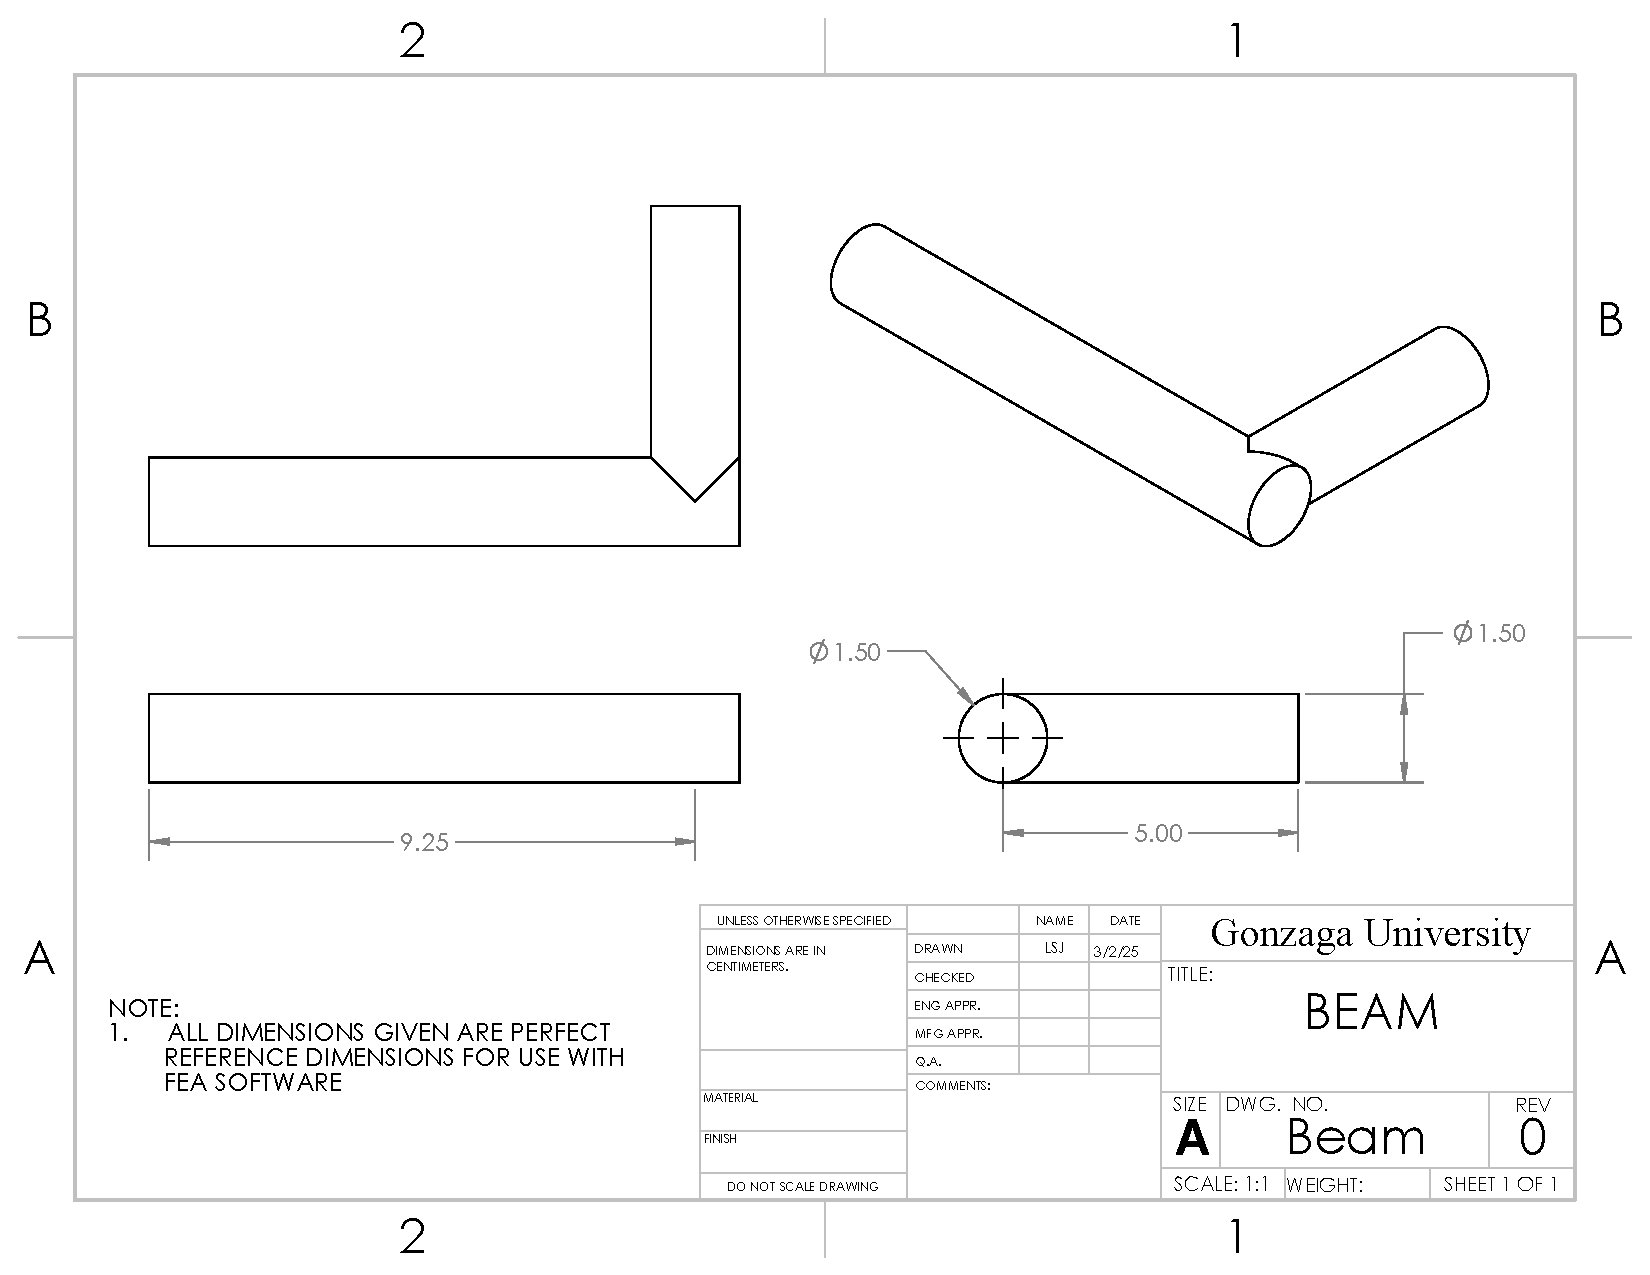
\includegraphics[height=0.75\textwidth]{figs/Beam.pdf}
            \end{minipage}%
            \begin{minipage}{.5\textwidth}
                \centering
                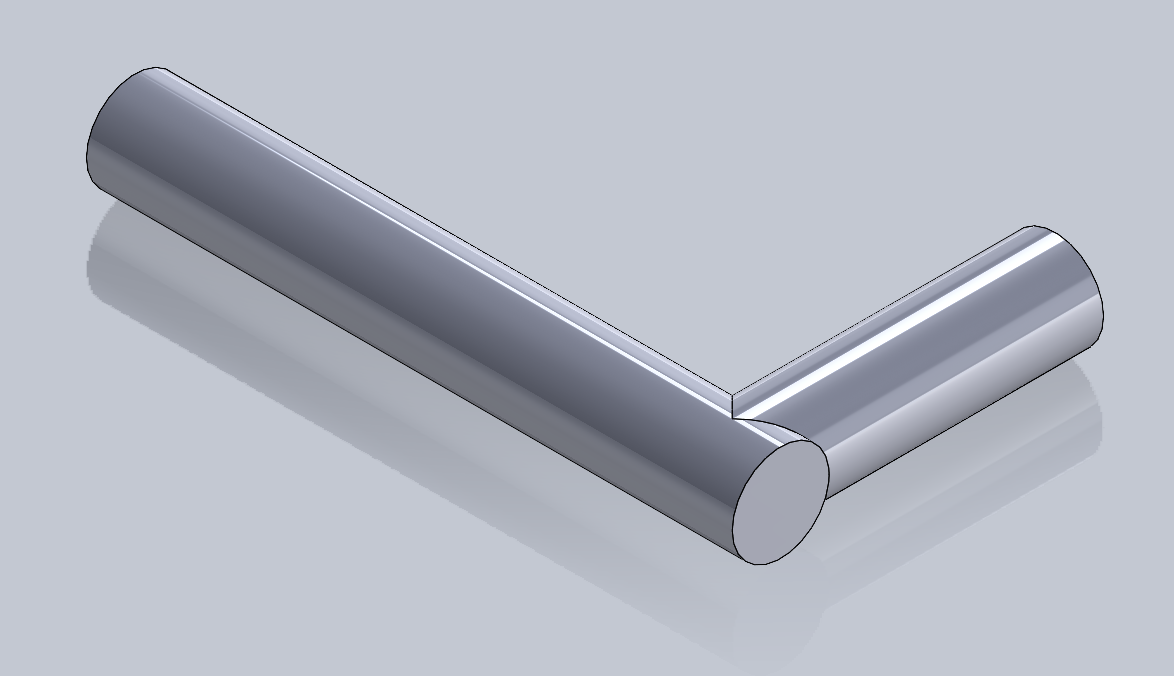
\includegraphics[height=0.65\textwidth]{figs/solidworks_isometric_cropped.png}
            \end{minipage}
            \caption{Beam Drawing}
        \end{figure}
    \end{frame}

    \begin{frame}{The Part: Material Properties}
        \begin{itemize}
            \item Structural Steel (Ansys material library)
            \item Evaluated at 22\textdegree\ Celcius
            \item Chosen as it's a typical material for this application
        \end{itemize}
        \begin{table}
            \scalebox{0.8}{
                \begin{tabular}{|c|c|c|} 
                    \hline
                    \textbf{Property} & \textbf{Value} & \textbf{Unit} \\
                    \hline\hline
                    Young's Modulus & 2E+11 & Pa\\ 
                    \hline
                    Poisson's Ratio & 0.3 &  \\
                    \hline
                    Bulk Modulus & 1.6667E+11 & Pa\\
                    \hline
                    Shear Modulus & 7.6223E+10 & Pa\\
                    \hline
                \end{tabular}
            }
            \caption{Structural Steel Properties}
        \end{table}
    \end{frame}

    \begin{frame}{Loading Conditions}
        \begin{itemize}
            \item Fixed at wall
            \item Forces, moments applied at centroid of circular cross sections
            \item Axes in Ansys to match those of problem description
        \end{itemize}
        \begin{figure}
            \centering
            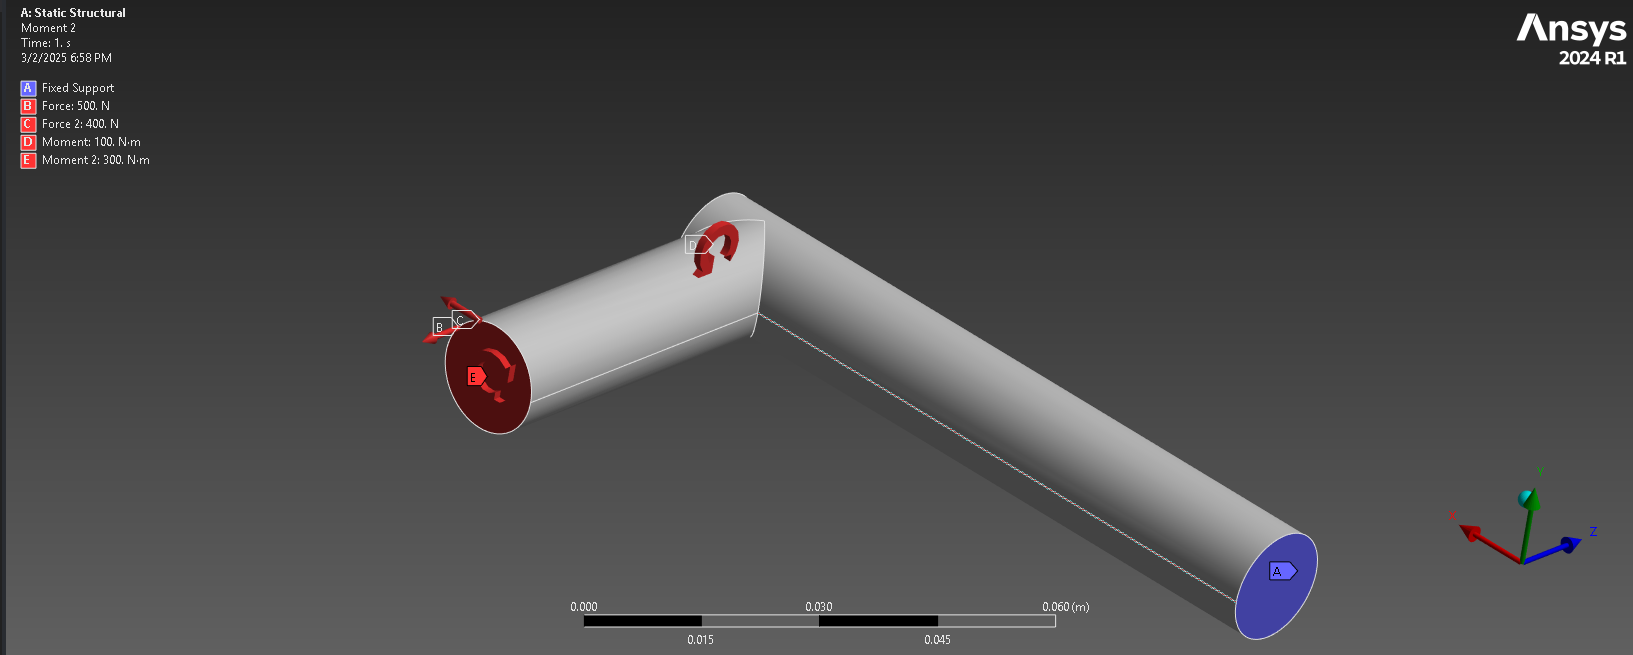
\includegraphics[scale=0.25]{figs/loading_condition_ansys_cropped.png}
            \caption{Loading Conditions}
        \end{figure}
    \end{frame}

    \begin{frame}{Load Steps} 
        \begin{itemize}
            \item Broke 400N shear into steps
            \item 4 steps, one second each
            \item Analyzed single node near element one for time analysis
        \end{itemize}

        \begin{figure}[H]
            \begin{minipage}{.5\textwidth}
                \centering
                \hspace{-15pt}
                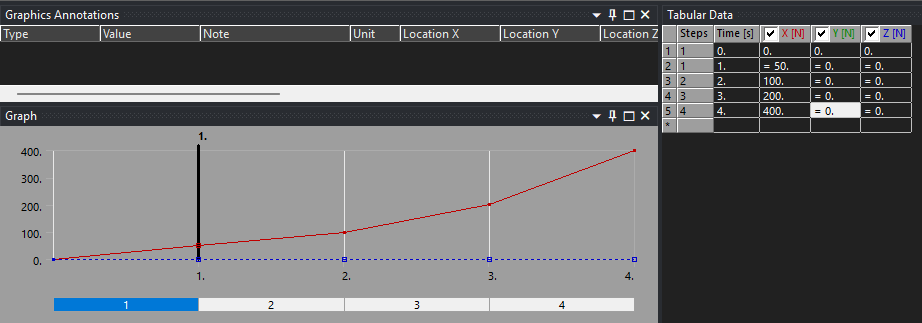
\includegraphics[height=0.4\textwidth]{figs/3E-3_Body_1E-3_Face/step_loading_graph_cropped.png}
            \end{minipage}%
            \begin{minipage}{.5\textwidth}
                \centering
                \hspace{15pt}
                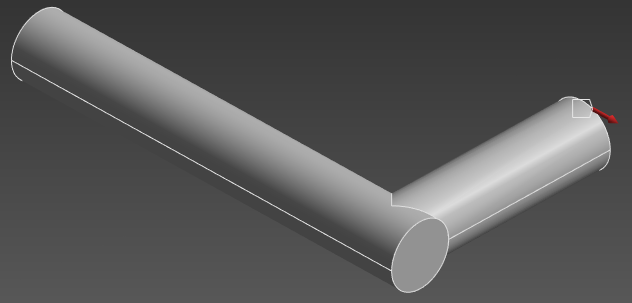
\includegraphics[height=0.4\textwidth]{figs/3E-3_Body_1E-3_Face/step_force_location_cropped.png}
            \end{minipage}
            \caption{Beam Drawing}
        \end{figure}
    \end{frame}

    \begin{frame}{Mesh Sizing: Chosen Mesh}
       \begin{itemize} 
           \item Used tetrahedrons for meshing 
            \item Decided to use 3E-3 m element size for body, 1E-3 m element size for face at wall for multi-step simulation
            \begin{itemize}
                \item Good balance between speed and accuracy, gives enough nodes to be away from boundary effects
            \end{itemize}
        \end{itemize}

        \begin{figure}[H]
            \centering
            \vspace{-17pt}
            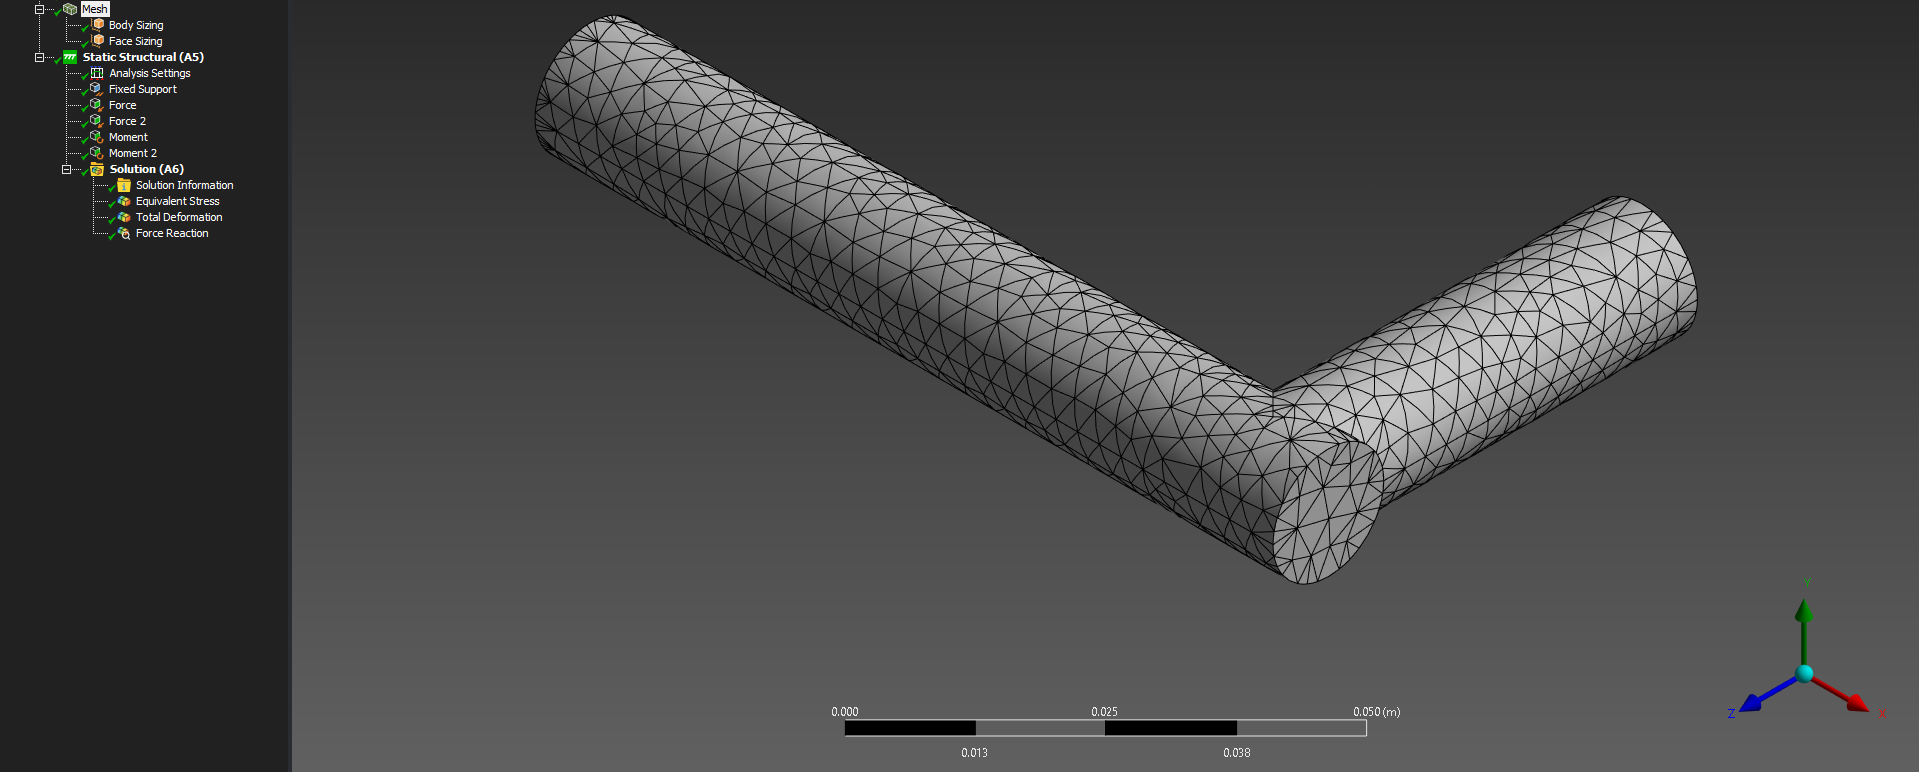
\includegraphics[scale=0.215]{figs/3E-3_Body_1E-3_Face/mesh_iso_ansys_cropped.png}
            \vspace{-20pt}
            \caption{Mesh}
        \end{figure}
    \end{frame}

    \begin{frame}{Mesh Sizing: Refinement Analysis}
       \centering
       \begin{itemize} 
           \item Experimented with meshing sizes for whole body, face attached to wall
           \item Compared against analytic result from Eq. \eqref{analytic_sln}
           \begin{itemize} 
                \item Similar to example shown in video
            \end{itemize}
           \item Smaller mesh size improvements largely obscured by difficulty setting probe in exact element one spot

       \end{itemize}

        \begin{figure} 
            \centering
            \begin{table}
                \hspace{-15pt}
                \scalebox{0.60}{
                    \begin{tabular}{|l|l|l|l|}
                        \hline
                        \textbf{Default Body Size (m)} & \textbf{Fixed Face Size (m)} & \textbf{von Mises stress (Pa)} & \textbf{Percent Error (\%)} \\
                        \hline\hline
                        5.81E-03 (default) & 5.81E-03 (default) & 9.36E+08 & 0.68\\ 
                        \hline
                        3.00E-03 & 1.00E-03 & 9.31E+08 & 1.21\\ 
                        \hline
                        2.50E-03 & 1.00E-03 & 9.21E+08 & 2.27\\
                        \hline
                        2.00E-03 & 7.50E-04 & 9.40E+08 & 0.25\\
                        \hline
                    \end{tabular}
                }
                \caption{Analysis of varying mesh element sizes}
                \label{tab:meshsizes}
            \end{table}
        \end{figure}
    \end{frame}


    \begin{frame}{Analyzed Results: Visual Representations} 
        \begin{figure}[H]
            \centering
            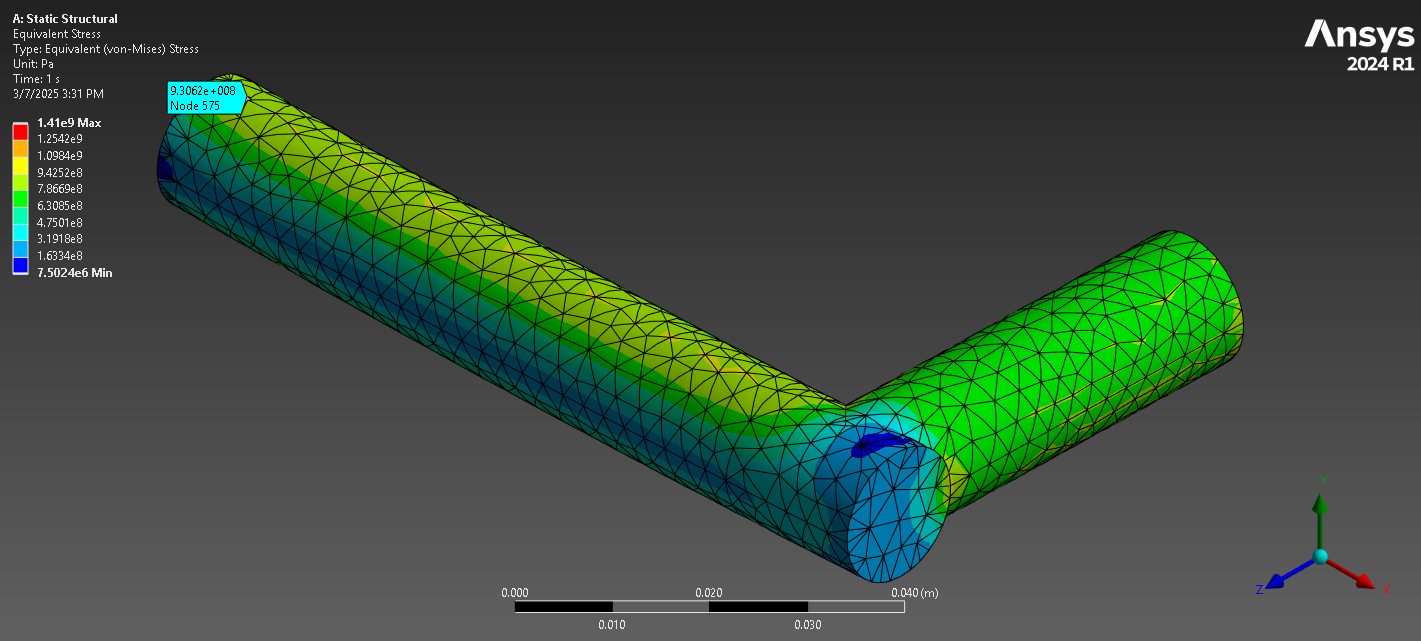
\includegraphics[height=0.325\textwidth]{figs/3E-3_Body_1E-3_Face/equiv_stress_cropped.png}
            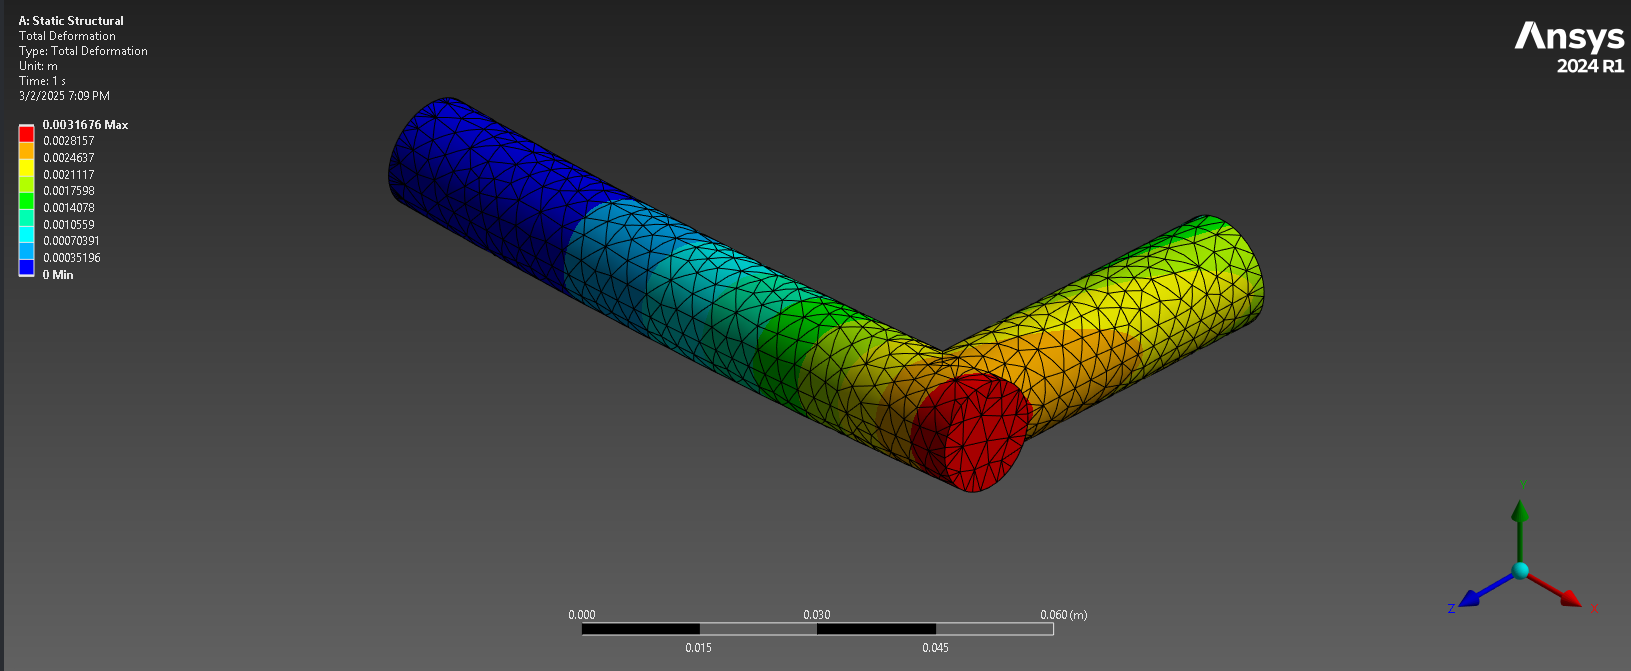
\includegraphics[height=0.30\textwidth]{figs/3E-3_Body_1E-3_Face/total_deformation_cropped.png}
            \caption{Solution Results}
        \end{figure}
    \end{frame}

    \begin{frame}{Analyzed Results: Step Response}
        \begin{table}[!ht]
            \scalebox{0.60}{
                \centering
                \begin{tabular}{|l|l|l|l|}
                \hline
                    \textbf{Time (s)} & \textbf{Load (N)} & \textbf{Stress (Pa)} & \textbf{Deflection (m/m)} \\
                    \hline\hline
                    1 & 50 & 7.47990E+06 & 3.74120E-05 \\ \hline
                    2 & 100 & 7.46090E+06 & 3.73170E-05 \\ \hline
                    3 & 200 & 7.44510E+06 & 3.72380E-05 \\ \hline
                    4 & 400 & 7.50240E+06 & 3.75250E-05 \\ \hline
                \end{tabular}
            }
            \caption{Stress, Strain Response to Changing Force}
        \end{table}
        \begin{figure}[H]
            \vspace{-15pt}
            \begin{tikzpicture}[scale=0.6]
                \begin{axis}[
                        xlabel =Load (N),
                        ylabel =Stress (Pa),
                    ]
                    \addplot
                    %table[y=Stress_Pa, x=Load_N, col sep=comma]{figs/loading_steps_table_no_spaces.csv}
                    % This is the loading steps table, I just modified a Min Working Example to 
                    %   get it to match
                    table[x=LoadN,y=StressPa,col sep=comma] {figs/table.csv}; 
                \end{axis}
            \end{tikzpicture}
            \vspace{-15pt}
            \caption{Stress vs. Load}
            \label{fig:stress_v_load}
        \end{figure}
    \end{frame}

    \begin{frame}{Analyzed Results: Analytical Values}
        \begin{itemize} 
            \item Have analytical solution for stress at top element of wall
            \item Use this value to validate FEA model
            \begin{equation}
                \sigma_{\textrm{eq}} = \sqrt{\frac{{\left(\sigma_1 - \sigma_2\right)}^2 + {\left(\sigma_2 - \sigma_3\right)}^2 + {\left(\sigma_3 - \sigma_1\right)}^2}{2}}
            \end{equation}
            \item Apply principle stresses solution from \href{https://github.com/A-Person7/a_design_class/blob/main/hw3/problem1.m}{here}
            \begin{equation}\label{analytic_sln}
                \hspace{-24pt}
                \resizebox{1\textwidth}{!}{$%
                    \sigma_{\textrm{eq}} = \sqrt{\frac{{\left(24.488\textrm{ MPa} - 0\textrm{ MPa}\right)}^2 + {\left(0\textrm{ MPa} - -929.903\textrm{ MPa}\right)}^2 + {\left(-929.903\textrm{ MPa} - 24.488\textrm{ MPa}\right)}^2}{2}} \approx 942.39\textrm{ MPa}
                $%
                }%
            \end{equation}
            \item Now have a way to check if Ansys simulation converges to sensical value
        \end{itemize}
    \end{frame}

    \begin{frame}{Analyzed Results: Computational and Analytical Comparison}
        \begin{itemize} 
            \item Saw within 1.5\% of expected theoretical value 
            \begin{itemize}
                \item see Table \ref{tab:meshsizes}
            \end{itemize}
            \item Simulation consistently underestimated stress
            \item Simulation reported maximum stress at `crook' of beam elbow joint
            \begin{itemize} 
                \item Have no analytical values there to compare to
            \end{itemize}
        \end{itemize}
    \end{frame}

    \begin{frame}{Sources of Error}
        \begin{itemize} 
            \item Most likely source of error is lack of mesh refinement
            \begin{itemize}
                \item Didn't specifically refine mesh around elbow joint
                \item Saw very high expected stress values at joint, higher than would expect
                \item Suggests that elbow joint mesh could be refined for better results
            \end{itemize}
            \item Should also check for discrepancies between loading conditions (e.g. force acting at centroid or at edge)
        \end{itemize}

        \begin{figure} 
            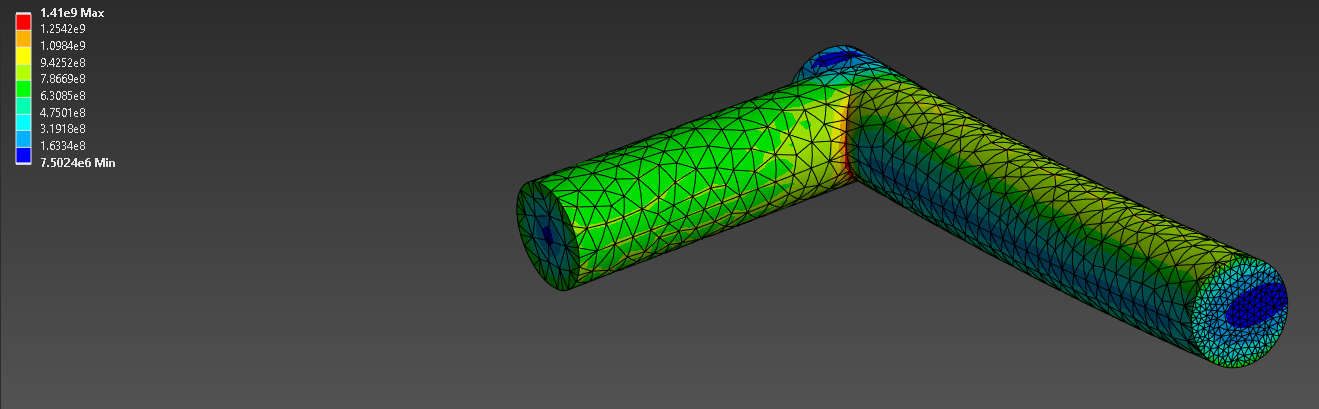
\includegraphics[scale=0.25]{figs/3E-3_Body_1E-3_Face/von_mises_eq_stress_better_view_cropped.png}
            \vspace{-7pt}
            \caption{Computed Stress at Elbow Joint (stress in units of Pa)}
        \end{figure}
    \end{frame}

    
    \begin{frame}{Breaking Ansys: Setup}
        \begin{itemize}
            \item Get impossible results by applying 0 displacement boundary conditions to edges, strong contradictory moments throughout the part
            \item Easier to get bad results in deflection analysis than stress analysis
        \end{itemize}

        \begin{figure}[H]
            \vspace{-9pt}
            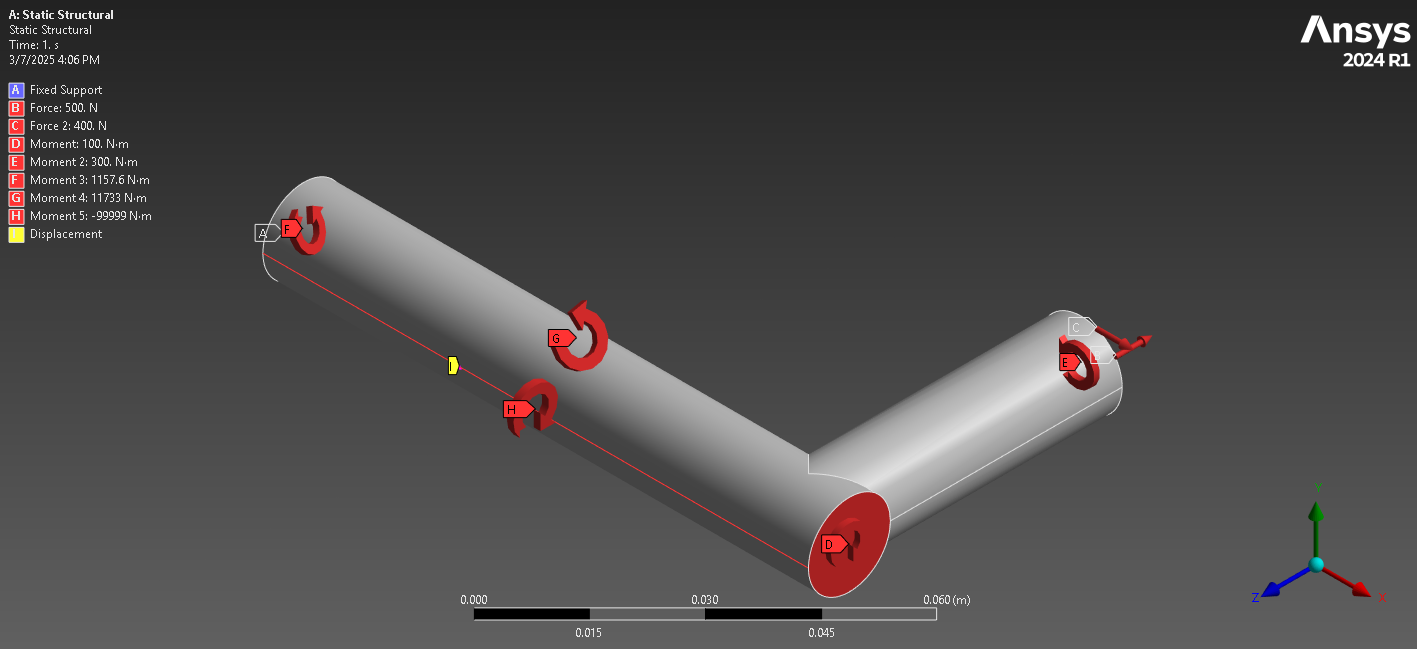
\includegraphics[scale=0.25]{figs/Broken_5.81E-3_All/loading_cropped.png}
            \vspace{-6pt}
            \caption{Loading Condition to `Break' Ansys}
        \end{figure}
  
    \end{frame}
    \begin{frame}{Breaking Ansys: Results}
        \begin{columns}[T]
            \begin{column}{0.65\textwidth}
                \vspace{10pt}
                \begin{itemize} 
                    \item Ansys fails to converge on valid beam
                    \item Beam is physically too large (see scale)
                \end{itemize} 
            \end{column}
            \begin{column}{0.5\textwidth}
                \begin{figure}[H]
                    \centering
                    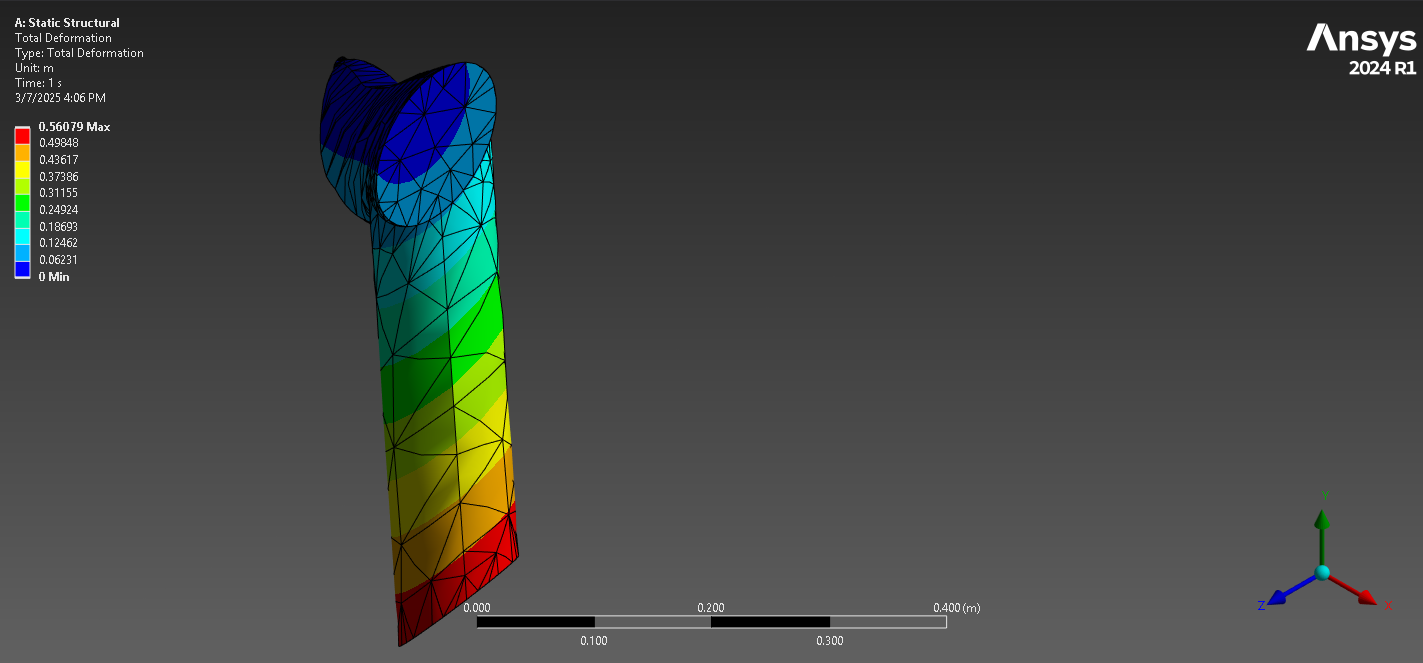
\includegraphics[scale=0.13]{figs/Broken_5.81E-3_All/iso_cropped.png}
                    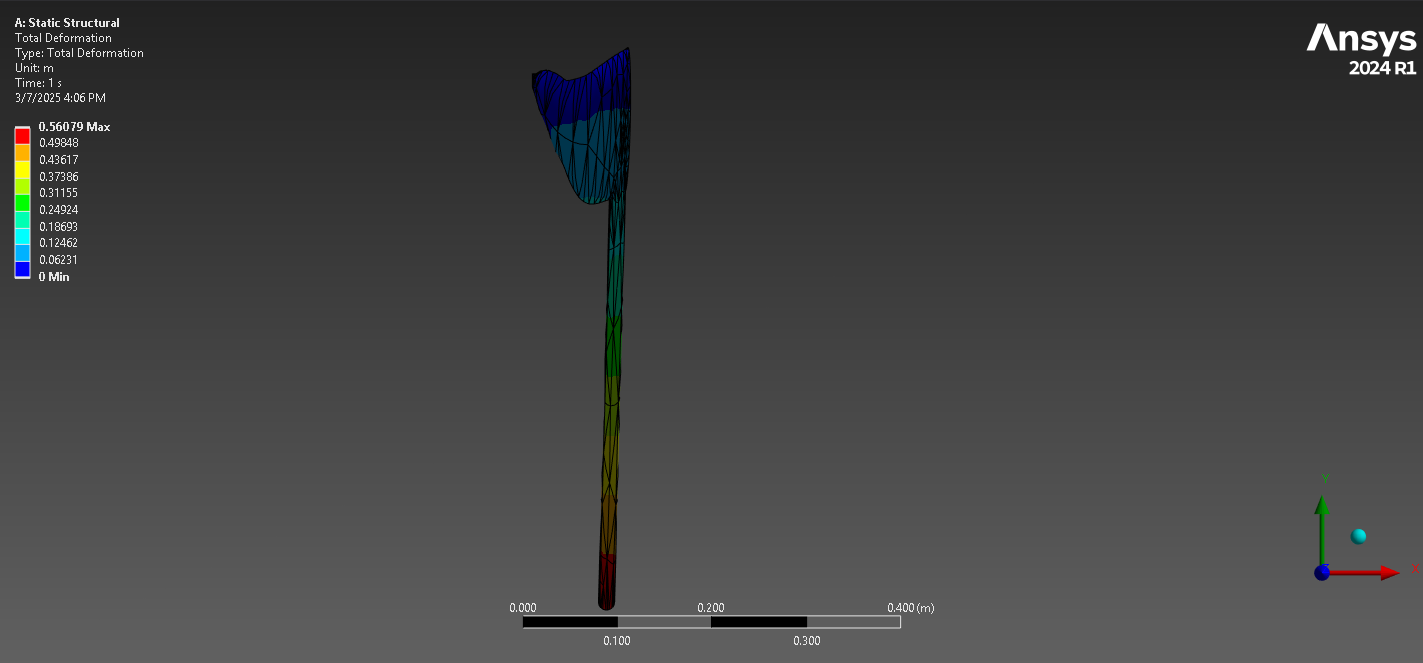
\includegraphics[scale=0.13]{figs/Broken_5.81E-3_All/z-axis_cropped.png}
                    \caption{Broken Beam}
                \end{figure}
            \end{column}
        \end{columns}
    \end{frame}
\end{document}
